\documentclass[letter]{article}
\usepackage{amsmath}
\usepackage{amsfonts}
\usepackage{amssymb}
\usepackage{ifthen}
\usepackage{fancyhdr}
\usepackage{graphicx}
\usepackage{subcaption}
\usepackage[shortlabels]{enumitem}

\newcommand{\fref}[1]{\textbf{Figure \ref{#1}}}

%%%
% Set up the margins to use a fairly large area of the page
%%%
\oddsidemargin=.2in
\evensidemargin=.2in
\textwidth=6in
\topmargin=0in
\textheight=9.0in
\parskip=.07in
\parindent=0in
\pagestyle{fancy}

%%%
% Set up the header
%%%
\newcommand{\setheader}[6]{
	\lhead{{\sc #1} {\sc #2}\\{} ({\small \it \today})}
	\rhead{
		{\bf #3} 
		\ifthenelse{\equal{#4}{}}{}{(#4)}\\
		{\bf #5}
		\ifthenelse{\equal{#6}{}}{}{(#6)}%
	}
}

\begin{document}
	\setheader{CSC490}{Module 1}{Ben Weisz}{}{Qiwen Hua}{}

	Note: We appologize for the length of the report but the figures take up quite a bit of space and add great value to the report.
	\section{Focal Loss \& Anisotropic Guassian}

	\subsection{Motivation}
	During our evaluation of the original algorithm designed for this module, we noticed the following two things:
	\begin{itemize}
		\item Among the top detections (detections with highest detection scores), we get a considerably lower precision score for the recall aggregates within the recall range of 0 and 0.1 than for range 0.1 to 0.2. What this tells us is that the false positive rates are higher among the top detections than in the 0.1 to 0.2 recall range. This can be seen in the 0.1 to 0.2 range on the horizontal axis in original PR Curve figure in report A for all values of $\tau$.
		\item As we sweep through the detection scores, the true and false positives are not evenly distributed in the aggregations. We see this in the fact that as we sweep through the detection scores the the curve has a noticeable negative slope. The reason that this may be bad is that we would ideally hope to see a higher rate of true positives even for lower detection scores. Since we get more false positives for the lower detection scores we can see that our current model does not match the ideal case.
		\item As we sweep through the detection scores we see that the recall scores tend to drop gradually as we decreases the scores. Ideally we would want to see these scores not decrease and then there be an abrupt decrease. This would mean that our model's recall is higher for more detections.
	\end{itemize}

	By tackling the above three problems we hope to decrease our model's false positive and false negative rates. This is important because by doing so we would increase both our recall and precision, thus leading to a better model overall.\\\\
	We will now present an overview of our technique, describing it in more detail in the techniques section. We use an anisotropic gaussian to model to model the vehicles for the target heatmap. We then use focal loss as our new loss function. This combination of the anisotropic gaussian and the focal loss function were chosen to hopefully allow the model to better orient the vehicles and because it focal loss helps the model focus on under represented classification cases.\\\\
	Alternatives to our techniques to tackling these issues will be presented at the end our our techniques section as future work. Both our methods and the alternative methods aim to decrease the false positive and negative rates among the detected vehicles.

	\subsection{Techniques}
	\textbf{Anistropic Gaussian:}\\
    The intuition behind using an anisotropic gaussian to model the the vehicle target heatmap is that we want the model to have a better understanding of the rotation and scale of the vehicles from the heatmap. An example output of of the target heatmap is show below in \fref{fig:aniso} During inference we use the heatmap to determine the point where a vehicle is located in the frame. We want to embue the predicted heatmap with orientation as this will help us better localize the vehicles, orient them and scale them. While we did get to implement the anisotropic gaussian, we did not have enough time to correctly make use of the predicted heatmap to help with orientation and scaling. The idea is, that with the predicted heatmap of oriented gaussians we fit a small GMM with one peak with a few iterations at infernce time to the region around the localized vehicle. Once fitted, the covariance matrix can be decomposed in to matricies for orientation and scale using singular value decomposition. These values for orientation and scale could then be combined with the regressed orientation and scale for a hopefully more accurate prediction.

	\begin{figure}[h]
		\begin{subfigure}[t]{0.49\textwidth}
			\centering
			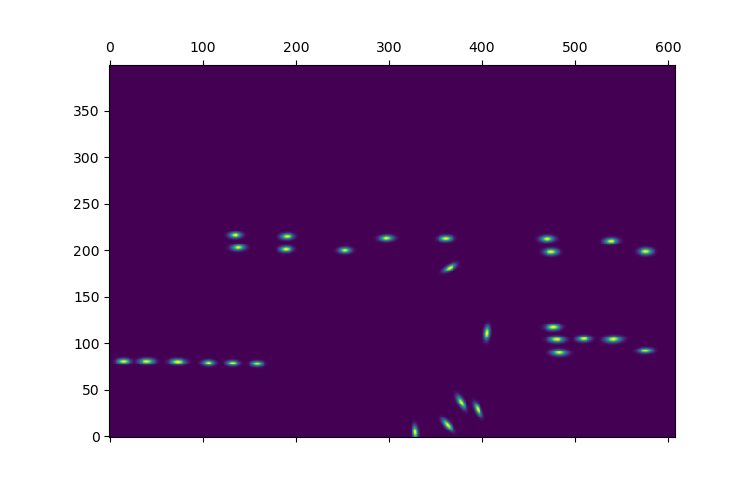
\includegraphics[scale=0.4]{images/aniso_target.png}
			\caption{Sample frame heatmap target.}
		\end{subfigure}
		\begin{subfigure}[t]{0.49\textwidth}
			\centering
			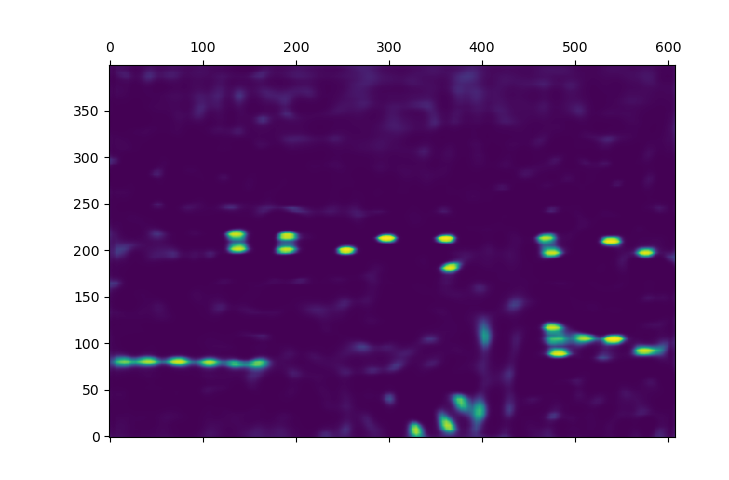
\includegraphics[scale=0.4]{images/aniso_pred.png}
			\caption{Sample frame heatmap prediction.}
		\end{subfigure}
		\vspace*{1mm}
		\caption{Heatmaps on frames from the training sequences}
		\label{fig:aniso}
	\end{figure}

	Breifly, we describe the method for generating the anisotropic gaussian targets. In order to properly capture the scale and orientation of vechiles in their location we wanted to gaurentee that at least 95\% of the point cloud points associated with a vehicle would be gauranteed to be within $2\sigma$ of the center location.
	\begin{align}
            2 \sigma_x &= \frac{s_x}{2}\\
			\sigma_x &= \frac{s_x}{4}
	\end{align}
	This gives us a value of $\sigma_x = \frac{s_x}{4}$ and $\sigma_y = \frac{s_y}{4}$ for the respective directions. These can then be placed along the diagonal of a matrix $S$ respectively with all other values being zero. The rotation matrix for the given yaw $\beta$ can be created using the standard 2 x 2 rotation matrix $R$. The covariance for the target gaussian can then be created as follows:
	\begin{align}
		\textstyle \sum = R S S R^\top
	\end{align}
	The anisotropic gaussian is then created using the standard multivariate gaussian formula, with the mean being the center locations of the vehicles.
	\begin{equation}
		\mathcal{N}(x, \textstyle \sum, \mu) = \frac{1}{(2\pi)^\frac{n}{2}}|\textstyle \sum|^{-\frac{1}{2}} exp (-\frac{1}{2}(x-\mu)^\top \textstyle \sum^{-1}(x - \mu))
	\end{equation}
	\textbf{Focal Loss:}\\
	Our intuition behind using focal loss is that we want to fix the inbalance between the types of examples the model sees and trains on. To stop model from localizing too many false positives and missing too may labels (minimizing false negatives) we weight these types of detections heavier in the loss function than ones for which the target does contain a vehicle in the heatmap and the model gets it somewhat right. This puts more emphasis on training the model to correctly classify these harder to detect cases.\\\\
	We use the Focal Loss suggested in \cite{objects-as-points} to compute the loss for our heatmap.
	\begin{equation}
		L_k = -\frac{1}{N} \sum_{xy} 
		\begin{cases} 
			(1 - \hat{Y}_{xy})^\alpha log (\hat{Y}_{xy}) & Y_{xy} > \tau\\
			(1 - Y_{xy})^\beta (\hat{Y}_{xy})^\alpha log(1 - \hat{Y}_{xy})& otherwise \\
		 \end{cases}
	\end{equation}
	Where $Y_{xy}, \hat{Y}_{xy}$ are the target and predicted heatmap outputs respectively, with $\tau$ representing a heatmap threshold and $\alpha, \beta$ being focal loss hyper parameters. $\tau, \alpha, \beta$ were tuned to $0.1$, $2.0$ and $4.0$ through testing and by recommendation in \cite{objects-as-points}. \\\\
	The regressed variables for scale, orientation and location are accounted for with an L1 loss function as recommended in \cite{objects-as-points}.\\\\
	These are then combined into the loss and weighted with parameters $\lambda_{k}, \lambda_{ori}, \lambda_{size}, \lambda_{loc}$ with tuned values of 100.0, 100.0, 1.0, 10.0 respectively.
	\begin{align}
		L = \lambda_k L_k + \lambda_{ori} L^1_{ori} + \lambda_{size} L^1_{size} + \lambda_{loc} L^1_{loc}
	\end{align}
	\textbf{Further Work:}\\
	One approach that could be taken to tackle some of the issues highlighted in the motivations would be to try to remove some labels in the raw data that have no overlapping point cloud data. In \fref{fig:false-positive} we can see that there are a lot of labels at the top of the frame were there is no point cloud data, thus making it hard for the model to learn these. In essence, using these labels currently trains the model to generate false positives as detections like these could be generated anywhere in the frame that has no points.\\\\
	To combat this, when building the targets, remove labels which have no point cloud data and train on the remaining labels.
	\begin{figure}[h]
		\centering
		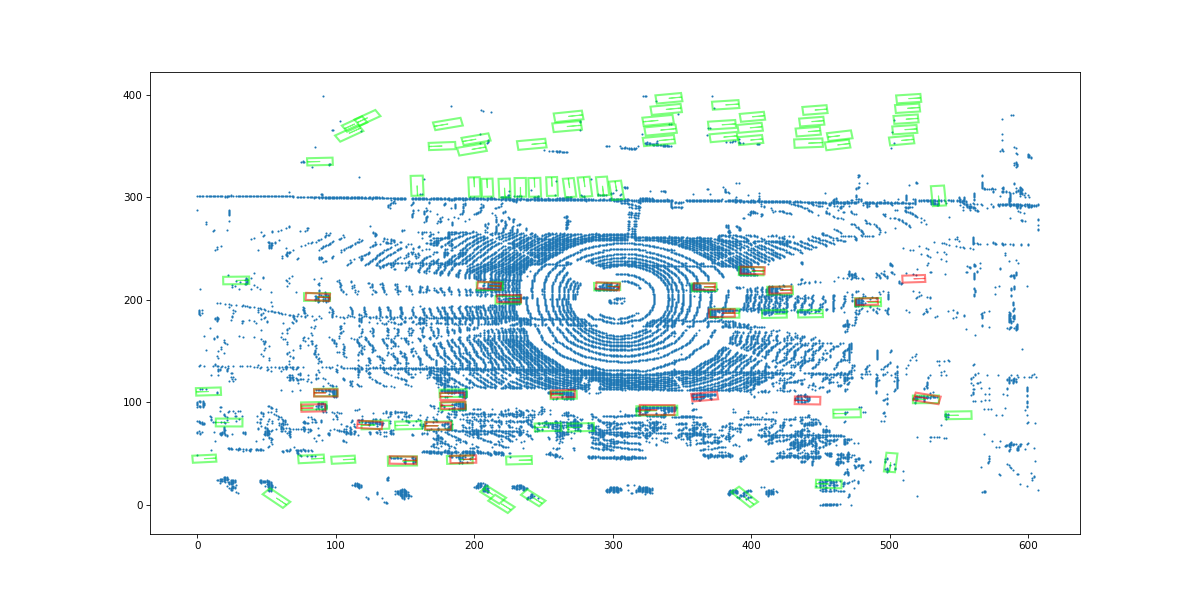
\includegraphics[scale=0.35]{images/false-positives.png}
		\caption{False positives along top of frame}
		\label{fig:false-positive}
	\end{figure}
	\newpage

	\subsection{Evaluation}
	Since one of our motivations was to decrease the number of false positives, negatives and increase the number of true positives, we analyzed the precision of the model by generating the PR curve for the new model using the same process as for the original model.\\\\
	Below we can see that by using focal loss we've managed to smooth out the jump in precision at among the highest detections (except for $\tau=2.0$). Overall, compared to the original model, the false positives are more distributed amongst the true positive detections. This can be seen in the charts below in the fact that the PR curves have a more flatline slope for recall ranges between 0.1 and 0.4.

	\begin{figure}[!h]
		\centering
		\begin{subfigure}[t]{0.4\textwidth}
			\centering
			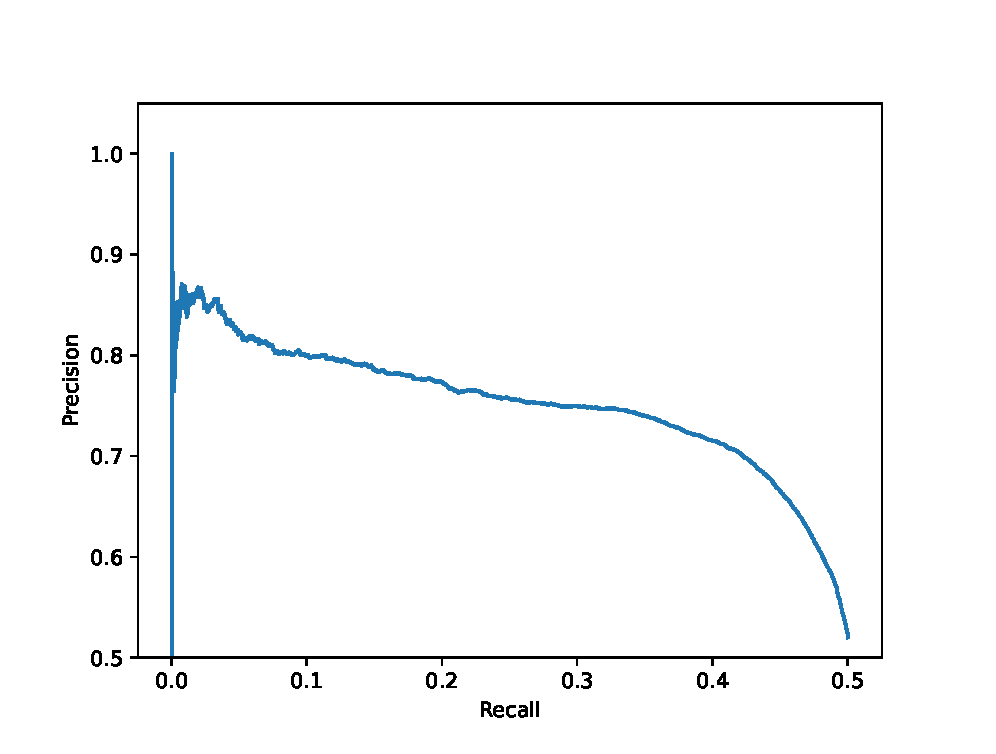
\includegraphics[width=\linewidth]{images/plot_tau_2_focal.eps}
			\caption{PR Curve with $\tau=2.0$}
		\end{subfigure}
		\begin{subfigure}[t]{0.4\textwidth}
			\centering
			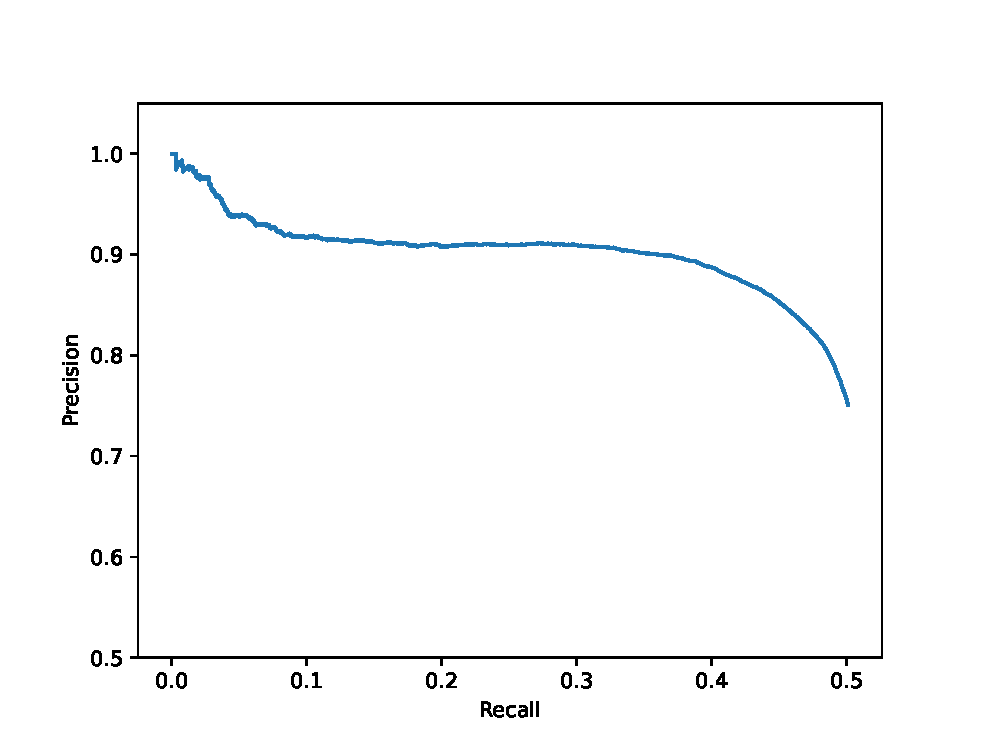
\includegraphics[width=\linewidth]{images/plot_tau_4_focal.eps}
			\caption{PR Curve with $\tau=4.0$}
		\end{subfigure}
		\vspace*{1mm}
	  
		\begin{subfigure}[t]{0.4\textwidth}
			\centering
			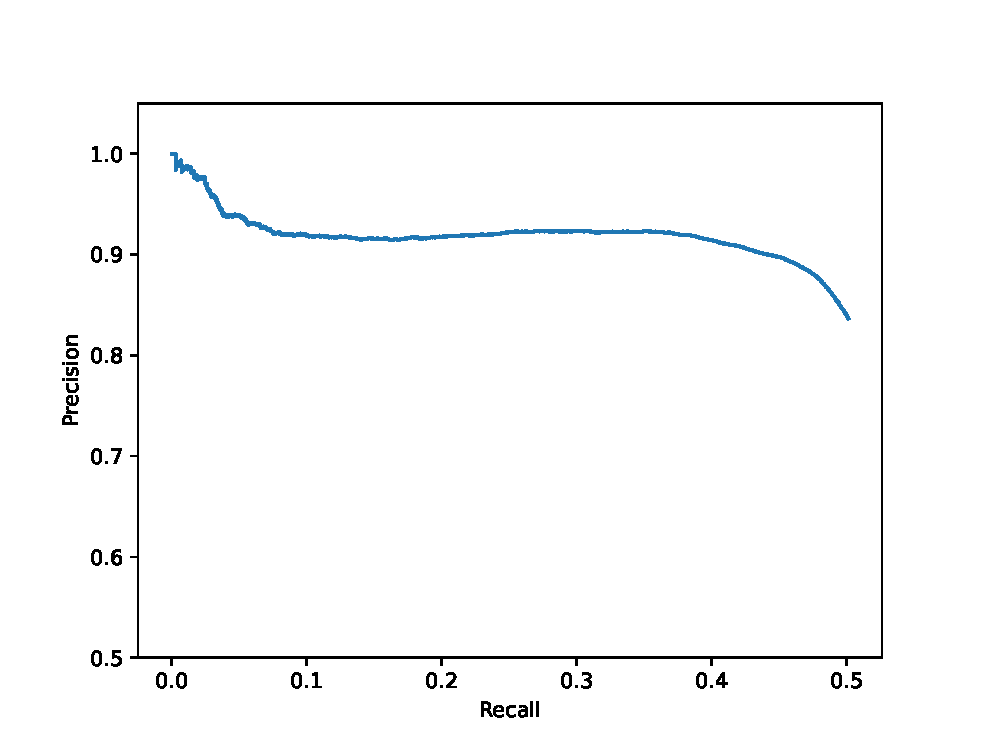
\includegraphics[width=\linewidth]{images/plot_tau_8_focal.eps}
			\caption{PR Curve with $\tau=8.0$}
		\end{subfigure}
		\begin{subfigure}[t]{0.4\textwidth}
			\centering
			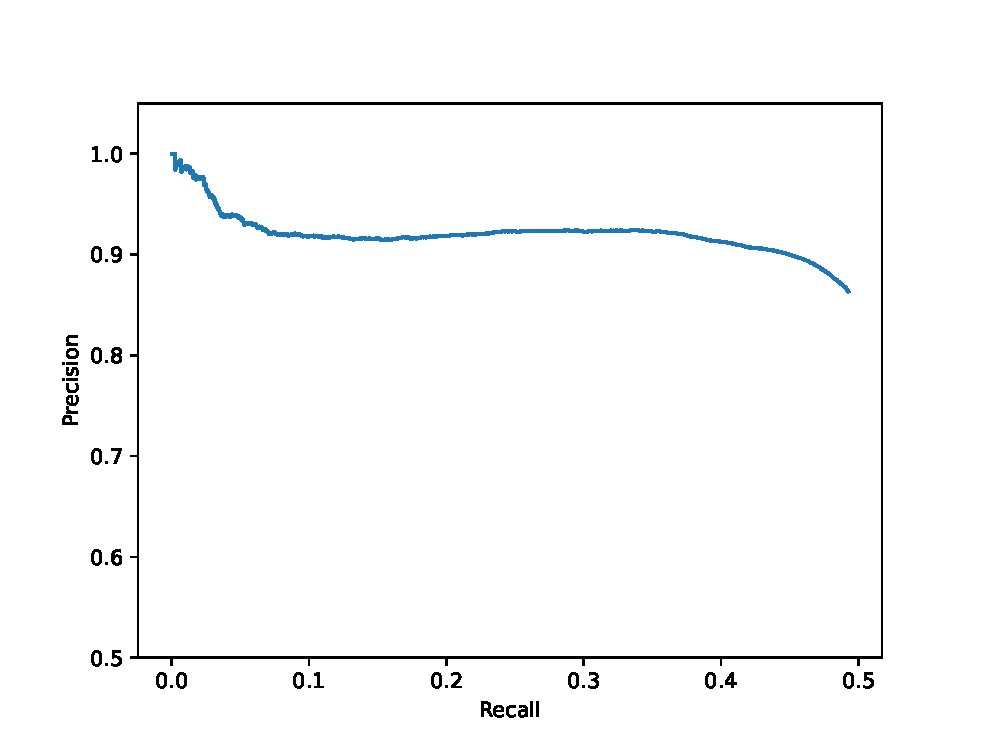
\includegraphics[width=\linewidth]{images/plot_tau_16_focal.eps}
			\caption{PR Curve with $\tau=16.0$}
		\end{subfigure}

		\caption{PR Curves for varying values of $\tau$ with focal loss}
		\label{fig:prcurvefocal}
	\end{figure}

	We can also see that the AP scores have also slightly increased for each value of $\tau$. Meaning that both the precision and recall have increased. This can be seen in $\textbf{Table \ref{tab:auc}}$.
	\begin{table}[!ht]
		\centering
		\begin{tabular}{|c|c|c|c|c|c|}
		\hline
		\textbf{Values of $\tau$} & 2.0 & 4.0 & 8.0 & 16.0 & \textbf{Mean} \\ \hline
		\textbf{AP for original Model} & 0.3792 & 0.4521 & 0.4609 & 0.4539 & 0.4365 \\ \hline
		\textbf{AP with Focal Loss} & 0.3944 & 0.4625 & 0.4702 & 0.4599 & 0.4468 \\ \hline
		\end{tabular}
		\caption{\label{tab:auc} AUC values for varying distance thresholds $\tau$}
	\end{table}

	In \fref{fig:comp-det}  we can qualitatively see that the new model is detecting more true positives than the old model quite accurately. 

	\begin{figure}[!h]
		\centering
		\begin{subfigure}[t]{0.49\textwidth}
			\centering
			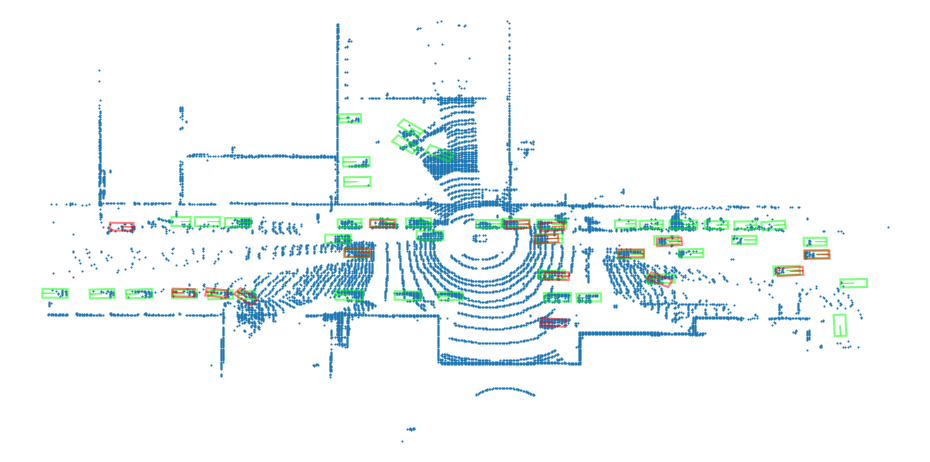
\includegraphics[width=\linewidth]{images/000.png}
			\caption{Detections of OLD model in test frame 000}
		\end{subfigure}
		\begin{subfigure}[t]{0.49\textwidth}
			\centering
			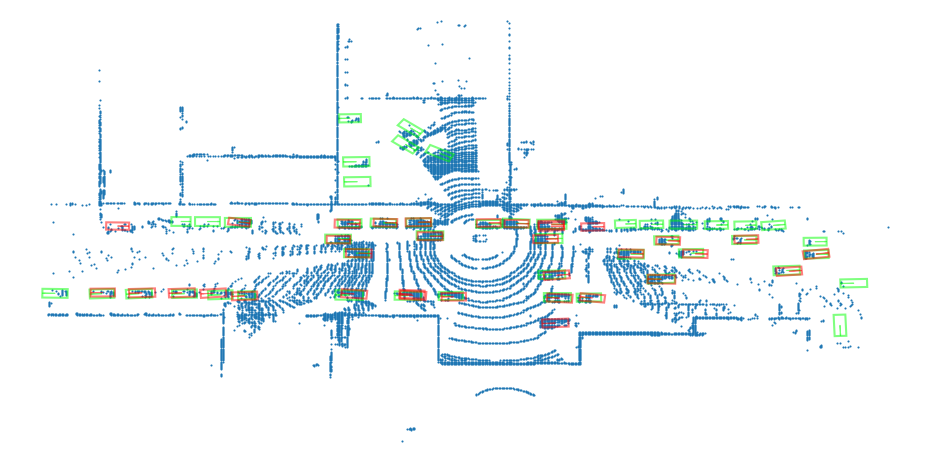
\includegraphics[width=\linewidth]{images/000-focal.png}
			\caption{Detections of NEW model in test frame 000}
		\end{subfigure}
		\caption{Comparision of detections for test 000.}
		\label{fig:comp-det}
	\end{figure}

	\subsection{Limitations}
	Since we did not get to completely implement the inferencing with the anisotropic gaussian we can see that there is a failure case that arises where objects that are further away cannot be properly orientated. An example of this can be seen in \fref{fig:failure} on the right hand side in the center. The green car is orientated parallel to the self driving car and but the detection says that it is roughly at a 45 degree angle.

	\begin{figure}[h]
		\centering
		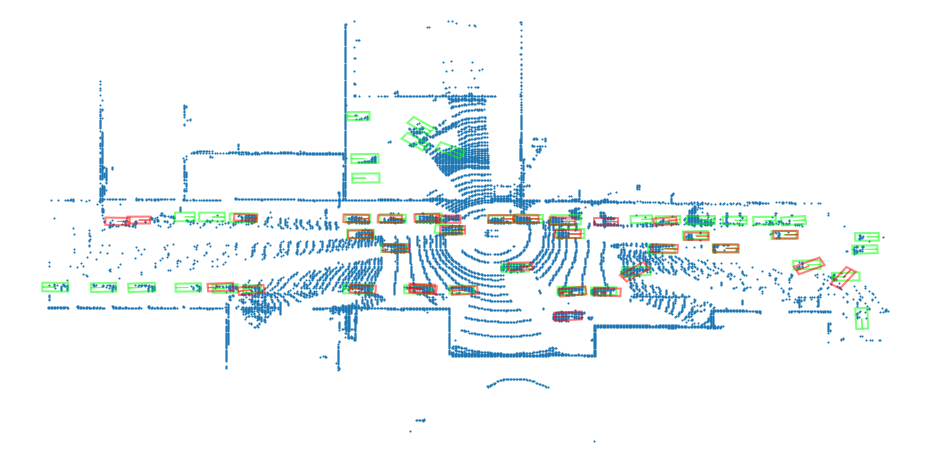
\includegraphics[scale=0.35]{images/failure.png}
		\caption{Detection orientation failure case.}
		\label{fig:failure}
	\end{figure}
	
	One potential improvement that could be made would be to multiple frames into the model at training time. Similar to how stereo vision allows one to triangulate objects in three dimensions, using multiple frames for one classification would allow the model to better understand where objects are, their size and their orientation. This could significantly improve the model's accuracy on far away objects as it can take multiple lidar measurements of these objects which is often needed due to the lack of data due to distance from the vehicle.

	\section{Multi-class Detector}

	\subsection{Motivation}

	\subsection{Techniques}

	\subsection{Evaluation}

	\subsection{Limitations}

	\begin{thebibliography}{9}
		\bibitem{objects-as-points}
		Xingyi Zhou and Dequan Wang and Philipp Kr{\"{a}}henb{\"{u}}hl (2019) \emph{Objects as Points}, CoRR.
	\end{thebibliography}
\end{document}

